\documentclass[%
    %handout
]{beamer}
\usepackage{graphicx} % For including single page pdfs
\usepackage{bm}       % bold math
\usepackage{pgffor}   % for loop
\usepackage{tikz}
\usepackage{multimedia}
\usepackage{layouts}
\usepackage{hyperref}
\usepackage{cambridge_lecture}

% todo 
% - Ligo actual data
% -define IMRPhenom, EOBNR


\newcommand{\lik}{\mathcal{L}}
\newcommand{\posterior}{\mathcal{P}}
\newcommand{\prior}{\pi}
\newcommand{\ev}{\mathcal{Z}}

\newcommand{\prob}{\mathrm{P}}

\newcommand{\PR}{\mathcal{P}_\mathcal{R}}
\newcommand{\Pknotj}[1]{\mathcal{P}_{#1}}
\newcommand{\Nknots}{N_\text{knots}}
\newcommand{\nlive}{n_\text{live}}

\newcommand{\movablecross}[1]{%
  \draw[->](#1) -- ++(0:\croslen);
  \draw[->](#1) -- ++(90:\croslen);
  \draw[->](#1) -- ++(180:\croslen);
  \draw[->](#1) -- ++(270:\croslen);
  \fill[red!70!black] (#1) circle (2pt);
}

\newcommand{\movablevert}[1]{%
  \draw[->](#1) -- ++(90:\croslen);
  \draw[->](#1) -- ++(270:\croslen);
  \fill[red!70!black] (#1) circle (2pt);
}

%Nested Sampling: an efficient and robust Bayesian inference tool for
%astrophysics and cosmology
%
%Nested sampling is an alternative MCMC technique for integrating and exploring
%probability distributions. It has become widely adopted in the field of
%cosmology as the de-facto tool for computing Bayesian evidences and sampling
%challenging a-priori unknown parameter spaces.
%
%In this talk, I will give an introduction to the principles of Bayesian model
%comparison and parameter estimation, an explanation of the theory of nested
%sampling, a survey of the current state-of-the art (MultiNest, PolyChord,
%DNest and Dynesty) and the future of the field. Throughout I will illustrate
%with examples of it's application in cosmology and astrophysics, ranging from
%inflationary physics to exoplanets.





\setbeamertemplate{navigation symbols}{} % Turn off that bottom bar


\title{Nested Sampling}
\subtitle{An efficient and robust Bayesian inference tool\\ for astrophysics and cosmology }
\author[Handley] % (optional, for multiple authors)
{Will Handley\\ \small{wh260@cam.ac.uk}}
\institute[University of Cambridge] % (optional)
{%
Astrophysics Group \\
Cavendish Laboratory \\
University of Cambridge
}
\date{May 9, 2018}

\usepackage{calculator}

\newcommand{\cols}[3][0.5]{%
    \SUBTRACT{1.}{#1}{\wdthb}
    \begin{columns}
        \begin{column}{#1\textwidth}
            #2
        \end{column}
        \begin{column}{\wdthb\textwidth}
            #3
        \end{column}
    \end{columns}
}

\newcommand{\figname}{}
\newenvironment{figright}[2][0.5]{%
    \renewcommand{\figname}{#2}
    \SUBTRACT{1.}{#1}{\wdthb}
    \begin{columns}
        \begin{column}{#1\textwidth}
        }{%
        \end{column}
        \begin{column}{\wdthb\textwidth}
            \includegraphics[width=\textwidth]{\figname}
        \end{column}
    \end{columns}
}

\newcommand{\dfigname}{}
\newenvironment{dfigright}[3][0.5]{%
    \renewcommand{\figname}{#2}
    \renewcommand{\dfigname}{#3}
    \SUBTRACT{1.}{#1}{\wdthb}
    \begin{columns}
        \begin{column}{#1\textwidth}
        }{%
        \end{column}
        \begin{column}{\wdthb\textwidth}
            \includegraphics[width=\textwidth]{\figname}
            \includegraphics[width=\textwidth]{\dfigname}
        \end{column}
    \end{columns}
}



\newenvironment{figleft}[2][0.5]{%
    \SUBTRACT{1.}{#1}{\wdthb}
    \begin{columns}
        \begin{column}{#1\textwidth}
            \includegraphics[width=\textwidth]{#2}
        \end{column}
        \begin{column}{\wdthb\textwidth}
        }{%
        \end{column}
    \end{columns}
}

\newenvironment{dfigleft}[3][0.5]{%
    \SUBTRACT{1.}{#1}{\wdthb}
    \begin{columns}
        \begin{column}{#1\textwidth}
            \includegraphics[width=\textwidth]{#2}
            \includegraphics[width=\textwidth]{#3}
        \end{column}
        \begin{column}{\wdthb\textwidth}
        }{%
        \end{column}
    \end{columns}
}


\newcounter{numimages}

\newenvironment{multifig}[1]{%
    \begin{frame}
        \pdfximage{#1}%
        \setcounter{numimages}{\the\pdflastximagepages}
        \addtocounter{numimages}{-1}

        \begin{tikzpicture}[remember picture, overlay]
            \foreach \pagenum in {1,...,\thenumimages} {%
                \node<handout:0|beamer:\pagenum>[anchor=center] at (current page.center) {
                \includegraphics[width=\textwidth,page=\pagenum]{#1}}; 
            }
            \addtocounter{numimages}{1}
            \node<handout:1|beamer:\thenumimages>[anchor=center] at (current page.center) {
            \includegraphics[width=\textwidth,page=\thenumimages]{#1}}; 
        \end{tikzpicture}
    }{%
    \end{frame}
}



\begin{document}

\begin{frame}
  \titlepage
\end{frame}

\section{Fitting a line to data}
\begin{frame}
    \frametitle{Motivating example}
    \framesubtitle{Fitting lines to data}
    \begin{figright}[0.4]{./figures/data_points.pdf}
        \begin{itemize}
            \item We have noisy data $D$
            \item We wish to fit a model $M$
            \item Functional form $y=f_M(x;\theta)$
            \item For example:
                \begin{align}
                     f_\text{linear}(x;\theta)&=a x + b       \nonumber\\
                     f_\text{quadratic}(x;\theta)&=a x^2 + b  \nonumber
                \end{align}
            \item Model parameters $\theta= (a,b)$
        \end{itemize}
    \end{figright}
\end{frame}

\begin{frame}
    \frametitle{$\chi^2$ best-fit}
    \framesubtitle{Fitting lines to data}
    \begin{figright}[0.4]{./figures/data_diff.pdf}
        \begin{itemize}
            \item For each parameter set $\theta$:
                \[
                    \chi^2(\theta) = \sum_i \left|y_i - f(x_i;\theta)\right|^2
                \]
            \item Minimise $\chi^2$ wrt $\theta$
        \end{itemize}
    \end{figright}
\end{frame}

\begin{frame}
    \frametitle{$\chi^2$ with non-uniform data errors}
    \framesubtitle{Fitting lines to data}
    \begin{figright}[0.4]{./figures/data.pdf}
        \begin{itemize}
            \item If data have non-uniform errors:
                \[
                    \chi^2(\theta) = \sum_i \frac{\left|y_i - f(x_i;\theta)\right|^2}{\sigma_i^2}
                \]
        \end{itemize}
    \end{figright}
\end{frame}

\begin{frame}
    \frametitle{Problems with $\chi^2$}
    \framesubtitle{Fitting lines to data}
    \begin{figright}[0.4]{./figures/data_diff_2.pdf}
        \begin{itemize}
            \item How do we differentiate between models
            \item Why square the errors? -- could take absolute:
                \[
                    \psi^2(\theta) = \sum_i \frac{\left|y_i - f(x_i;\theta)\right|}{\sigma_i}
                \]
            \item Where does this approach even come from?
        \end{itemize}
    \end{figright}
\end{frame}

\begin{frame}
    \frametitle{Multivariate probability}
    \begin{itemize}
        \item Marginalisation:
            \begin{equation*}
                P(x) = \int P(x,y) dy
            \end{equation*}
        \item Conditioning:
            \begin{equation*}
                P(y|x) = \frac{P(x,y)}{P(x)} = \frac{P(x,y)}{\int P(x,y) dy}
            \end{equation*}
        \item De-Conditioning:
            \begin{equation*}
                P(x|y) P(y) = P(x,y)
            \end{equation*}
        \item Bayes theorem:
            \begin{equation*}
                P(y|x) = \frac{P(x|y) P(y)}{P(x)}
            \end{equation*}
            \begin{center}
                ``To flip a conditional $P(x|y)$, you first de-condition on $y$,\\ and then re-condition on $x$.''
            \end{center}
    \end{itemize}
\end{frame}

\begin{frame}
    \frametitle{Probability distributions}
    \framesubtitle{Fitting lines to data}
    \begin{figright}[0.6]{./figures/data_diff_1.pdf}
        \begin{itemize}
            \item The probability of observing a datum:
                \[
                    P(y_i | \theta,M) = \frac{1}{\sqrt{2\pi}\sigma_i}\exp\left({-\frac{|y_i-f(x_i;\theta)|^2}{2\sigma_i^2}}\right)
                \]
            \item The probability of observing the data:
                \begin{align}
                    P(D | \theta,M) &= \prod_i \frac{1}{\sqrt{2\pi}\sigma_i}\exp\left({-\frac{|y_i-f(x_i;\theta)|^2}{2\sigma_i^2}}\right) \nonumber\\
                    &=  \frac{1}{\prod_i\sqrt{2\pi}\sigma_i}\exp\sum_i{-\frac{|y_i-f(x_i;\theta)|^2}{2\sigma_i^2}} \nonumber\\
                    &\propto e^{-\chi^2(\theta)/2}
                    \nonumber
                \end{align}
        \end{itemize}
    \end{figright}
\end{frame}



\begin{frame}
    \frametitle{Maximum likelihood}
    \framesubtitle{Fitting lines to data}
    \begin{figleft}[0.6]{./figures/data_diff.pdf}
        \begin{itemize}
            \item Minimising $\chi^2(\theta)$  is equivalent to maximising $P(D|\theta,M) \propto e^{-\chi^2(\theta)/2}$
            \item $P(D|\theta,M)$ is called the Likelihood $L=L(\theta)$ of the parameters $\theta$
            \item ``Least squares'' $\equiv$ ``maximum likelihood'' \\(if data are gaussian).
        \end{itemize}
    \end{figleft}
\end{frame}

\begin{frame}
    \frametitle{Bayesian inference}
    \begin{itemize}
        \item Likelihood $L=P(D|\theta,M)$ is undeniably correct.
        \item Frequentists construct inference techniques purely from this function.
        \item The trend is cosmology is to work with a Bayesian approach.
        \item What we want are things like $P(\theta|D,M)$ and $P(M|D)$.
        \item To invert the conditionals, we need Bayes theorem:
            \begin{align}
                P(\theta|D,M) &= \frac{P(D|\theta,M) P(\theta|M)}{P(D|M)} \nonumber\\
                P(M|D) &= \frac{P(D|M) P(M)}{P(D)} \nonumber
            \end{align}
    \end{itemize}
\end{frame}

\begin{frame}
    \frametitle{Terminology}
    \framesubtitle{Bayesian inference}
    \begin{align}
        P(\theta|D,M) &= \frac{P(D|\theta,M) P(\theta|M)}{P(D|M)} \nonumber\\
        \text{Posterior} &= \frac{\text{Likelihood}\times\text{Prior}}{\text{Evidence}} \nonumber
    \end{align}
    \begin{align}
        P(M|D) &= \frac{P(D|M) P(M)}{P(D)} \nonumber\\
        \text{Model probability} &= \frac{\text{Evidence}\times\text{Model Prior}}{\text{Normalisation}} \nonumber
    \end{align}
\end{frame}

\begin{frame}
    \frametitle{The prior}
    \framesubtitle{Example: Biased coins}
    \begin{itemize}
        \item Need to define the \textbf{Prior} $P(\theta)$ --- probability of the bias, given no data
        \item Represents our knowledge of parameters before the data -- subjective
        \item Frequentists view this as a flaw in Bayesian inference. 
        \item Bayesians view this as an advantage
        \item Fundamental rule of Inference:\pause\\
            \vfill
            \begin{center}
                \Large You cannot extract information from data\\ without making assumptions 
            \end{center}
            \vfill
        \item All Bayesians do is make them explicit
        \item Any method that claims it is ``objective'' is simply hiding them
    \end{itemize}
\end{frame}

\begin{frame}
    \frametitle{Parameter estimation}
    \framesubtitle{Bayesian inference}
    \begin{figright}[0.3]{./figures/parameters.pdf}
        \begin{itemize}
            \item We may use $P(\theta|D,M)$ to inspect whether a model looks reasonable
        \end{itemize}
        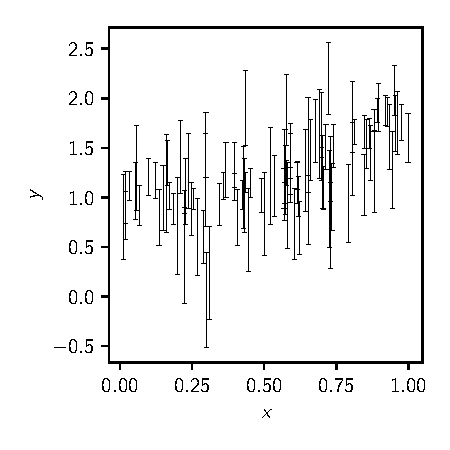
\includegraphics[width=\textwidth]{./figures/data.pdf}
    \end{figright}
\end{frame}

\begin{frame}
    \frametitle{Predictive posterior}
    \begin{figright}[0.4]{./figures/fgivenx.pdf}
        More useful to plot:
        \begin{align}
        &P(y|x) = \nonumber\\
        &\int P(y|x,\theta) P(\theta) d\theta \nonumber
        \end{align}
        (all conditioned on $D,M$)
    \end{figright}
\end{frame}

\begin{frame}
    \frametitle{Model comparison}
    \framesubtitle{Bayesian inference}
    \begin{figright}[0.33]{./figures/evidences_log.pdf}
        \begin{itemize}
            \item We may use the Bayezian evidence $Z$ to determine whether a model is reasonable.
            \item $Z = P(D|M) = \int P(D|M,\theta)P(\theta|M)d\theta$
            \item Normally assume uniform model priors $Z \propto P(M|D)P(M)$.
        \end{itemize}
    \end{figright}
\end{frame}
\begin{frame}
    \frametitle{Model comparison}
    \framesubtitle{Bayesian inference}
    \begin{figright}[0.33]{./figures/evidences_lin.pdf}
        \begin{itemize}
            \item We may use the Bayezian evidence $Z$ to determine whether a model is reasonable.
            \item $Z = P(D|M) = \int P(D|M,\theta)P(\theta|M)d\theta$
            \item Normally assume uniform model priors $Z \propto P(M|D)P(M)$.
        \end{itemize}
    \end{figright}
\end{frame}

\begin{frame}
    \frametitle{Line fitting (context)}
    \begin{figright}[0.5]{./figures/supernovae.pdf}
        \begin{itemize}
            \item Whilst this model seems a little trite\ldots
            \item\ldots determining polynomial indices \\$\equiv$ determining cosmological material content:
        \end{itemize}
    \end{figright}
        \[
            {\left( \frac{H}{H_0} \right)}^2 = 
            \Omega_\text{r} {\left( \frac{a_0}{a} \right)}^4+
            \Omega_\text{m} {\left( \frac{a_0}{a} \right)}^3+
            \Omega_k {\left( \frac{a_0}{a} \right)}^2+
            \Omega_\Lambda
            \]
\end{frame}



\begin{frame}
    \frametitle{Quantifying error with Probability}

    \begin{itemize}
        \item As scientists, we are used to seeing error bars on results.
        \item Age of the universe ({\em Planck\/}): 
         \[13.73\pm 0.12\:\text{billion years old.}\]
        \item Masses of LIGO GW150914 binary merger: 
        \[m_1 = 39.4^{+5.5}_{-4.9}\:M_\odot,\qquad m_2 = 30.9^{+4.8}_{-4.4}\:M_\odot \]
        \item These are called {\em credible intervals}, state that we are e.g.\ $90\%$ confident of the value lying in this range.
        \item More importantly, these are {\em summary statistics}.
    \end{itemize}
\end{frame}

\begin{frame}
    \frametitle{LIGO binary merger}
    \begin{columns}
        \begin{column}{0.65\textwidth}
            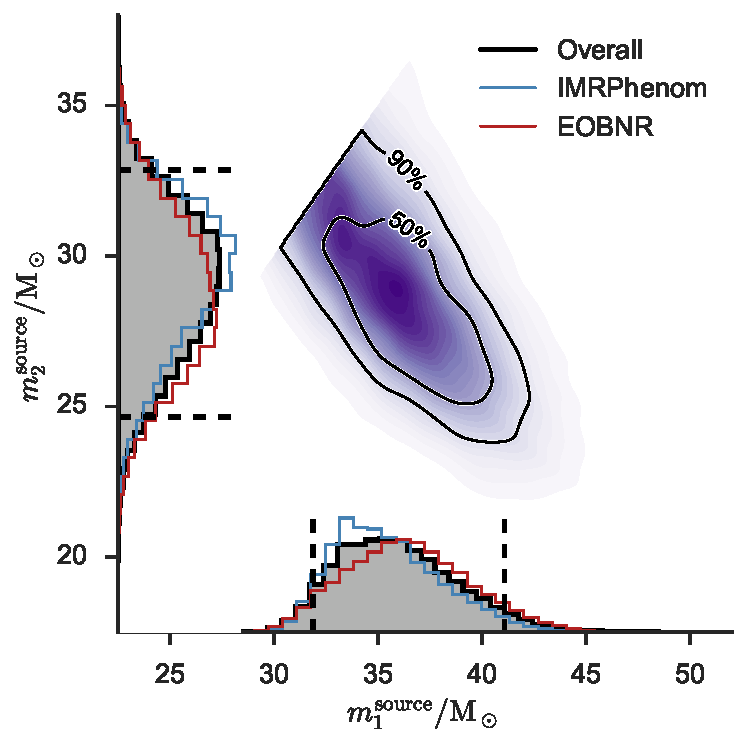
\includegraphics[width=\textwidth]{./figures/ligo_m1_m2.pdf}
        \end{column}
        \begin{column}{0.35\textwidth}
            \begin{itemize}
                \item Summary statistics summarise a full probability distribution.
                \item One goal of inference is to produce these probability distributions.
            \end{itemize}
        \end{column}
    \end{columns}
\end{frame}

\begin{frame}
    \frametitle{Theory}
    \framesubtitle{Extended example of inference: LIGO}
    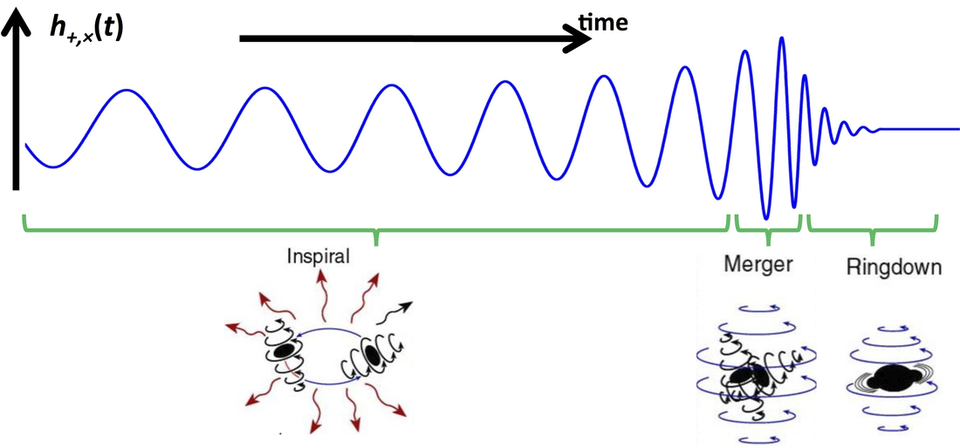
\includegraphics[width=\textwidth]{./figures/ligo_schematic.png}
\end{frame}

\begin{frame}
    \frametitle{The parameters $\Theta$ of the model $M$}
    \framesubtitle{Extended example of inference: LIGO}
    Theoretical signal depends on:
    \begin{itemize}
        \item $m_1, m_2$: mass of binary
        \item $\theta, \phi$: sky location
        \item $r$: luminosity distance 
        \item $\Phi_c, t_c$: phase and time of coalescence
        \item $i, \theta_\text{sky}$: inclination and angle on sky (orbital parameters)
    \end{itemize}
\end{frame}



\begin{frame}
    \frametitle{Posterior $\mathcal{P}$}
    \framesubtitle{Extended example of inference: LIGO}
    \begin{itemize}
        \item Cannot plot the full posterior distribution:
            \[\mathcal{P}(\Theta) \equiv P(m_1,m_2,\theta,\phi,r,\Phi_c, t_c, i, \theta_\text{sky}|D,M)\]
        \item Can plot 1D and 2D {\em marginalised\/} distributions e.g:
            \begin{align}
            &P(m_1,m_2|D,M)=\nonumber\\&\int P(m_1,m_2,\theta,\phi,r,\Phi_c, t_c, i, \theta_\text{sky}|D,M) \,d\theta \,d\phi \,dr \,d\Phi_c \,d t_c \,d i \,d\theta_\text{sky}\nonumber
            \end{align}
        \item May do this for each pair of parameters
        \item Generates a {\em triangle plot}
    \end{itemize}
\end{frame}


\begin{frame}
    \frametitle{Posterior $\mathcal{P}$}
    \framesubtitle{Extended example of inference: LIGO}
    \begin{figleft}[0.65]{./figures/ligo_full.pdf}
		\begin{itemize}
          \item Does give insight
          \item Not the full picture
		\end{itemize}
    \end{figleft}
\end{frame}


\begin{frame}
    \frametitle{Sampling}
    \framesubtitle{How to describe a high-dimensional posterior}

	\begin{figright}{./figures/ligo_m1_m2.pdf}
		\begin{itemize}
          \item In high dimensions, posterior $\posterior$ occupies a vanishingly small region of the prior $\prior$.
          \item Gridding is doomed to failure for $D\gtrsim4$.
          \item {\em Sampling\/} the posterior is an excellent compression scheme.
		\end{itemize}
	\end{figright}
 
\end{frame}
%
\begin{frame}
    \frametitle{Why do sampling?}
    \framesubtitle{Marginalisation over the posterior}

    \begin{itemize}
        \item Set of $N$ samples $S = \{\Theta^{(i)}: i=1,\ldots N:\: \Theta^{(i)}\sim\mathcal{P}\}$
        \item Mean mass: \[
                \bar{m}_1 \equiv\langle m_1\rangle_\mathcal{P}
                \only<1>{\equiv \int m_1 P(\theta|D,M) d\theta }
                \only<2>{\approx \frac{1}{N}\sum_{i=1}^N m_1^{(i)}}
                \only<3>{\approx \frac{\sum_{i=1}^N w^{(i)} m_1^{(i)}}{\sum_{i=1}^N w^{(i)}}}
            \]
        \item Mass covariance: \[
                \mathrm{Cov}(m_1,m_2)
            \only<1>{\equiv \int (m_1-\bar{m}_1)(m_2-\bar{m}_2) P(\theta|D,M) d\theta }
                \only<2>{\approx \frac{1}{N}\sum_{i=1}^N (m_1^{(i)}-\bar{m}_1)(m_2^{(i)}-\bar{m}_2)}
                \only<3>{\approx \frac{\sum_{i=1}^N w^{(i)} (m_1^{(i)}-\bar{m}_1)(m_2^{(i)}-\bar{m}_2)}{\sum_{i=1}^N w^{(i)}}}
            \]
        \item Marginalised samples: Just ignore the other coordinates.
        \item N.B. Typically have {\em weighted\/} samples
    \end{itemize}
\end{frame}
%
\begin{frame}
    \frametitle{Parameter estimation}
    \begin{itemize}
        \item The name of the game is therefore drawing samples $S$ from the posterior $\mathcal{P}$ with the minimum number of likelihood calls.
        \item Gridding is doomed to failure in high dimensions.
        \item Enter Metropolis Hastings.
    \end{itemize}
\end{frame}



\section{Metropolis Hastings}


\begin{frame}
  \frametitle{Metropolis Hastings} 
  \begin{itemize}
      
    \item Turn the $N$-dimensional problem into a one-dimensional one.
      \begin{enumerate}
        \item Propose random step
        \item If uphill, make step\ldots
          
        \item \ldots otherwise sometimes make step. 
      \end{enumerate}
  \end{itemize}
\end{frame}

\begin{frame}
  \frametitle{Metropolis Hastings} 
  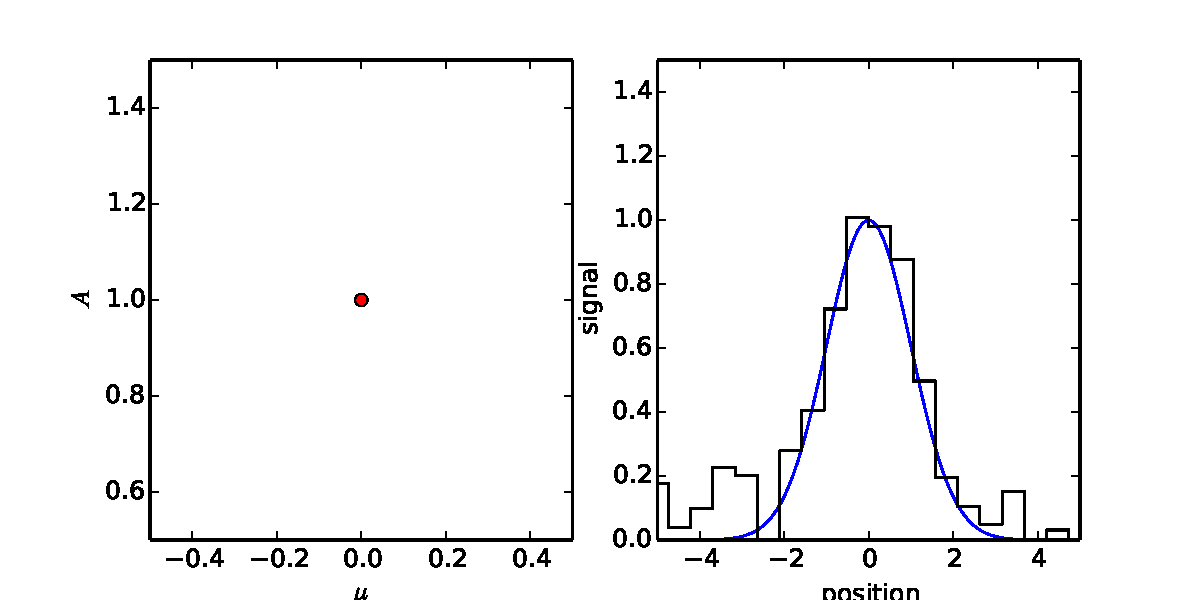
\includegraphics[width=\textwidth]{movies/MCMC_0.pdf}
\end{frame}
\begin{frame}
  \frametitle{Metropolis Hastings} 
  \movie[width=\textwidth,height=0.52\textwidth]{}{movies/MCMC.mp4}
\end{frame}
\begin{frame}
  \frametitle{Metropolis Hastings} 
  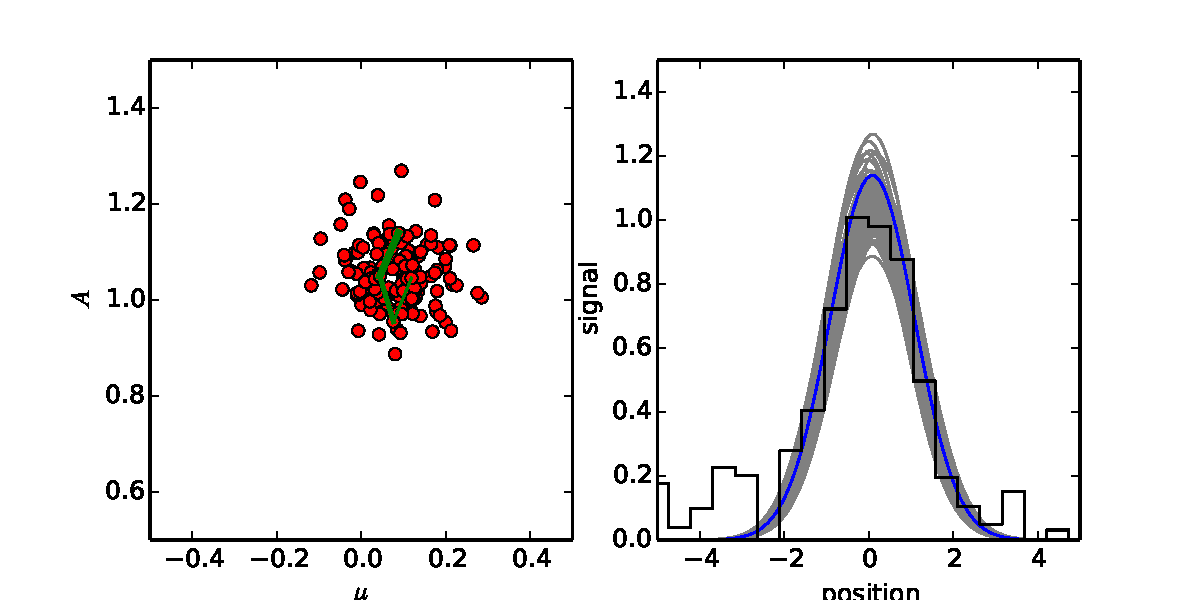
\includegraphics[width=\textwidth]{movies/MCMC_1.pdf}
\end{frame}




\begin{frame}
  \frametitle{Metropolis Hastings} 
  \framesubtitle{Struggles with\ldots}
  \pause
  \begin{enumerate}
      \item Burn in
      \item Multimodality
      \item Correlated Peaks
      \item Phase transitions
  \end{enumerate}
\end{frame}

\begin{frame}
  \frametitle{Hamiltonian Monte-Carlo} 
  \begin{itemize}
      \item Key idea: Treat $\log L(\Theta)$ as a potential energy
      \item Guide walker under ``force'': \[F(\Theta) =\nabla \log L(\Theta)\]
      \item Walker is naturally ``guided'' uphill
      \item Conserved quantities mean efficient acceptance ratios.
      \item stan is a fully fledged, rapidly developing programming language with HMC as a default sampler.
  \end{itemize}
\end{frame}


\begin{frame}
  \frametitle{Ensemble sampling} 
  \begin{itemize}
      \item Instead of one walker, evolve a set of $n$ walkers.
      \item Can use information present in ensemble to guide proposals.
      \item emcee: affine invariant proposals.
      \item emcee is not the only (or even best) affine invariant approach.
  \end{itemize}
\end{frame}

\begin{frame}
  \frametitle{The fundamental issue with all of the above} 

  \begin{itemize}
    \item They don't give you evidences!
  \begin{align}
    \ev 
    &= \prob(D|M) 
    \nonumber\\
    &= \int\prob(D|\Theta,M)\prob(\Theta|M) d\Theta 
    \nonumber\\
    &= \left\langle \lik \right\rangle_\prior
    \nonumber
  \end{align}
    \item MCMC fundamentally explores the posterior, and cannot average over the prior.
    \item Thermodynamic annealing 
    \begin{itemize}
        \item Suffers from same tuning issues as MCMC
    \end{itemize}
    \item Nearest neighbor volume estimation (Heavens arXiv:1704.03472)
    \begin{itemize}
        \item Does not scale to high dimensions $D\gtrsim15$.
    \end{itemize}
  \end{itemize}
 
\end{frame}

\section{Nested Sampling}

\begin{frame}
  \frametitle{Nested Sampling} 
  \framesubtitle{John Skilling's alternative to traditional MCMC!} 

  \begin{itemize}
    \item Nested sampling is a completely different way of sampling. 
    \item Uses ensemble sampling to compress prior to posterior.
  \end{itemize}
  
  New procedure: 

  
  Maintain a set $S$ of $n$ samples, which are sequentially updated:

  \begin{description}
      
    \item[$S_0$:] Generate $n$ samples uniformly over the space (from the prior $\prior$). 
      
    \item[$S_{n+1}$:] Delete the lowest likelihood sample in $S_{n}$, and replace it with a new uniform sample with higher likelihood
  \end{description}

  
  Requires one to be able to uniformly within a region, subject to a {\em hard likelihood constraint}.

\end{frame}



\begin{frame}
  \frametitle{Nested Sampling}
  \framesubtitle{Graphical aid}
\foreach \pagenum in {1,...,38} {%
  \includegraphics<\pagenum>[width=\textwidth,page=\pagenum]{figures/nested_sampling}
}
\end{frame}

\begin{frame}
  \frametitle{Nested sampling} 

  \begin{itemize}
    \item The set of dead points are posterior samples with an appropriate weighting factor
    \item They can also be used to calculate evidences, since it sequentially updates the priors.
  \end{itemize}
 
\end{frame}

\begin{frame}
  \frametitle{Nested Sampling}
  \framesubtitle{Calculating evidences}
  \foreach \pagenum in {1,...,16} {%
      \includegraphics<\pagenum>[width=\textwidth,page=\pagenum]{figures/lesbesgue}
  }
\end{frame}



\begin{frame}
  \frametitle{Sampling from a hard likelihood constraint} 

  
  \begin{quote}
    ``It is not the purpose of this introductory paper to develop the technology of navigation within such a volume. We merely note that exploring a hard-edged likelihood-constrained domain should prove to be neither more nor less demanding than exploring a likelihood-weighted space.''
    
   {\hfill --- John Skilling}
  \end{quote}

  \begin{itemize}
      
    \item Most of the work in NS to date has been in attempting to implement a hard-edged sampler in the NS meta-algorithm.
  \end{itemize}
 
\end{frame}

\begin{frame}
\frametitle{MultiNest }
  \framesubtitle{arXiv:0809.3437 arXiv:0704.3704 arXiv:1306.2144}
  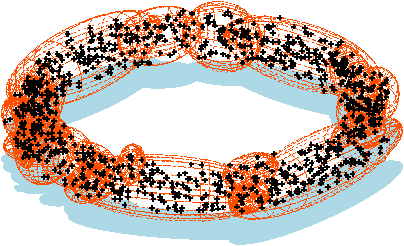
\includegraphics[width=\textwidth]{figures/multinest.pdf}
\end{frame}

\begin{frame}
  \frametitle{PolyChord}
  \framesubtitle{arXiv:1502.01856 arXiv:1506.00171}
  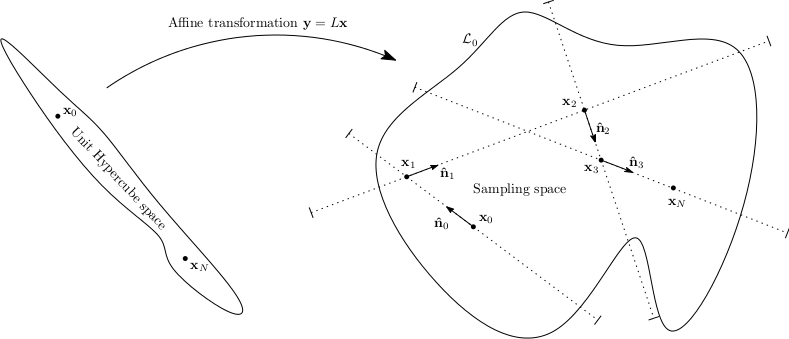
\includegraphics[width=\textwidth]{figures/polychord.png}
\end{frame}

\begin{frame}
  \frametitle{Diffusive nested sampling}
  \framesubtitle{arXiv:0912.2380}
  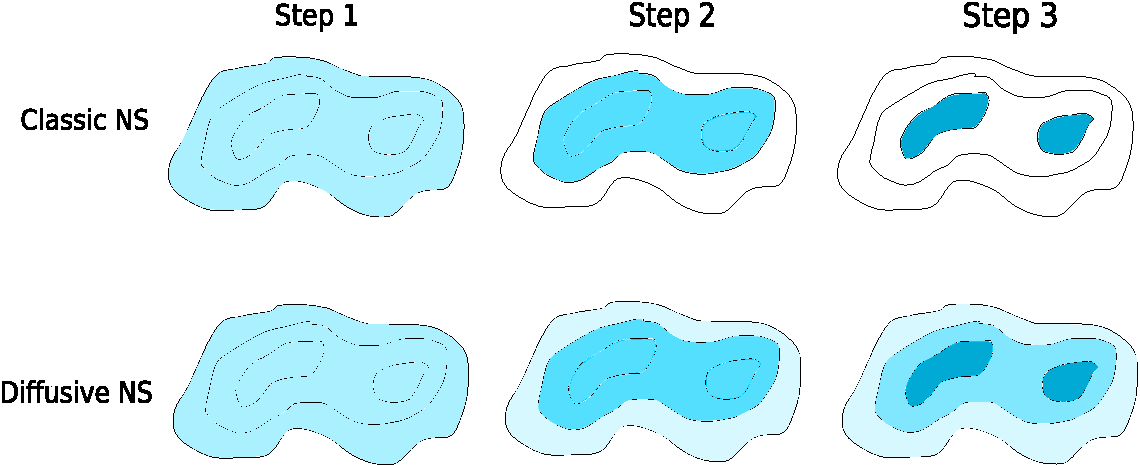
\includegraphics[width=\textwidth]{figures/dnest.pdf}
\end{frame}

\begin{frame}
\frametitle{PolyChord vs MultiNest}
\begin{itemize}
    \item MultiNest excels in low dimensions $D<10-20$.
    \item PolyChord can go up to $\sim 150$.
    \item Crossover is problem dependent
    \item PolyChord can also exploit fast-slow hierarchy
\end{itemize}
\end{frame}

\begin{frame}
  \frametitle{Exoplanets}
  \framesubtitle{Nested sampling in action}
  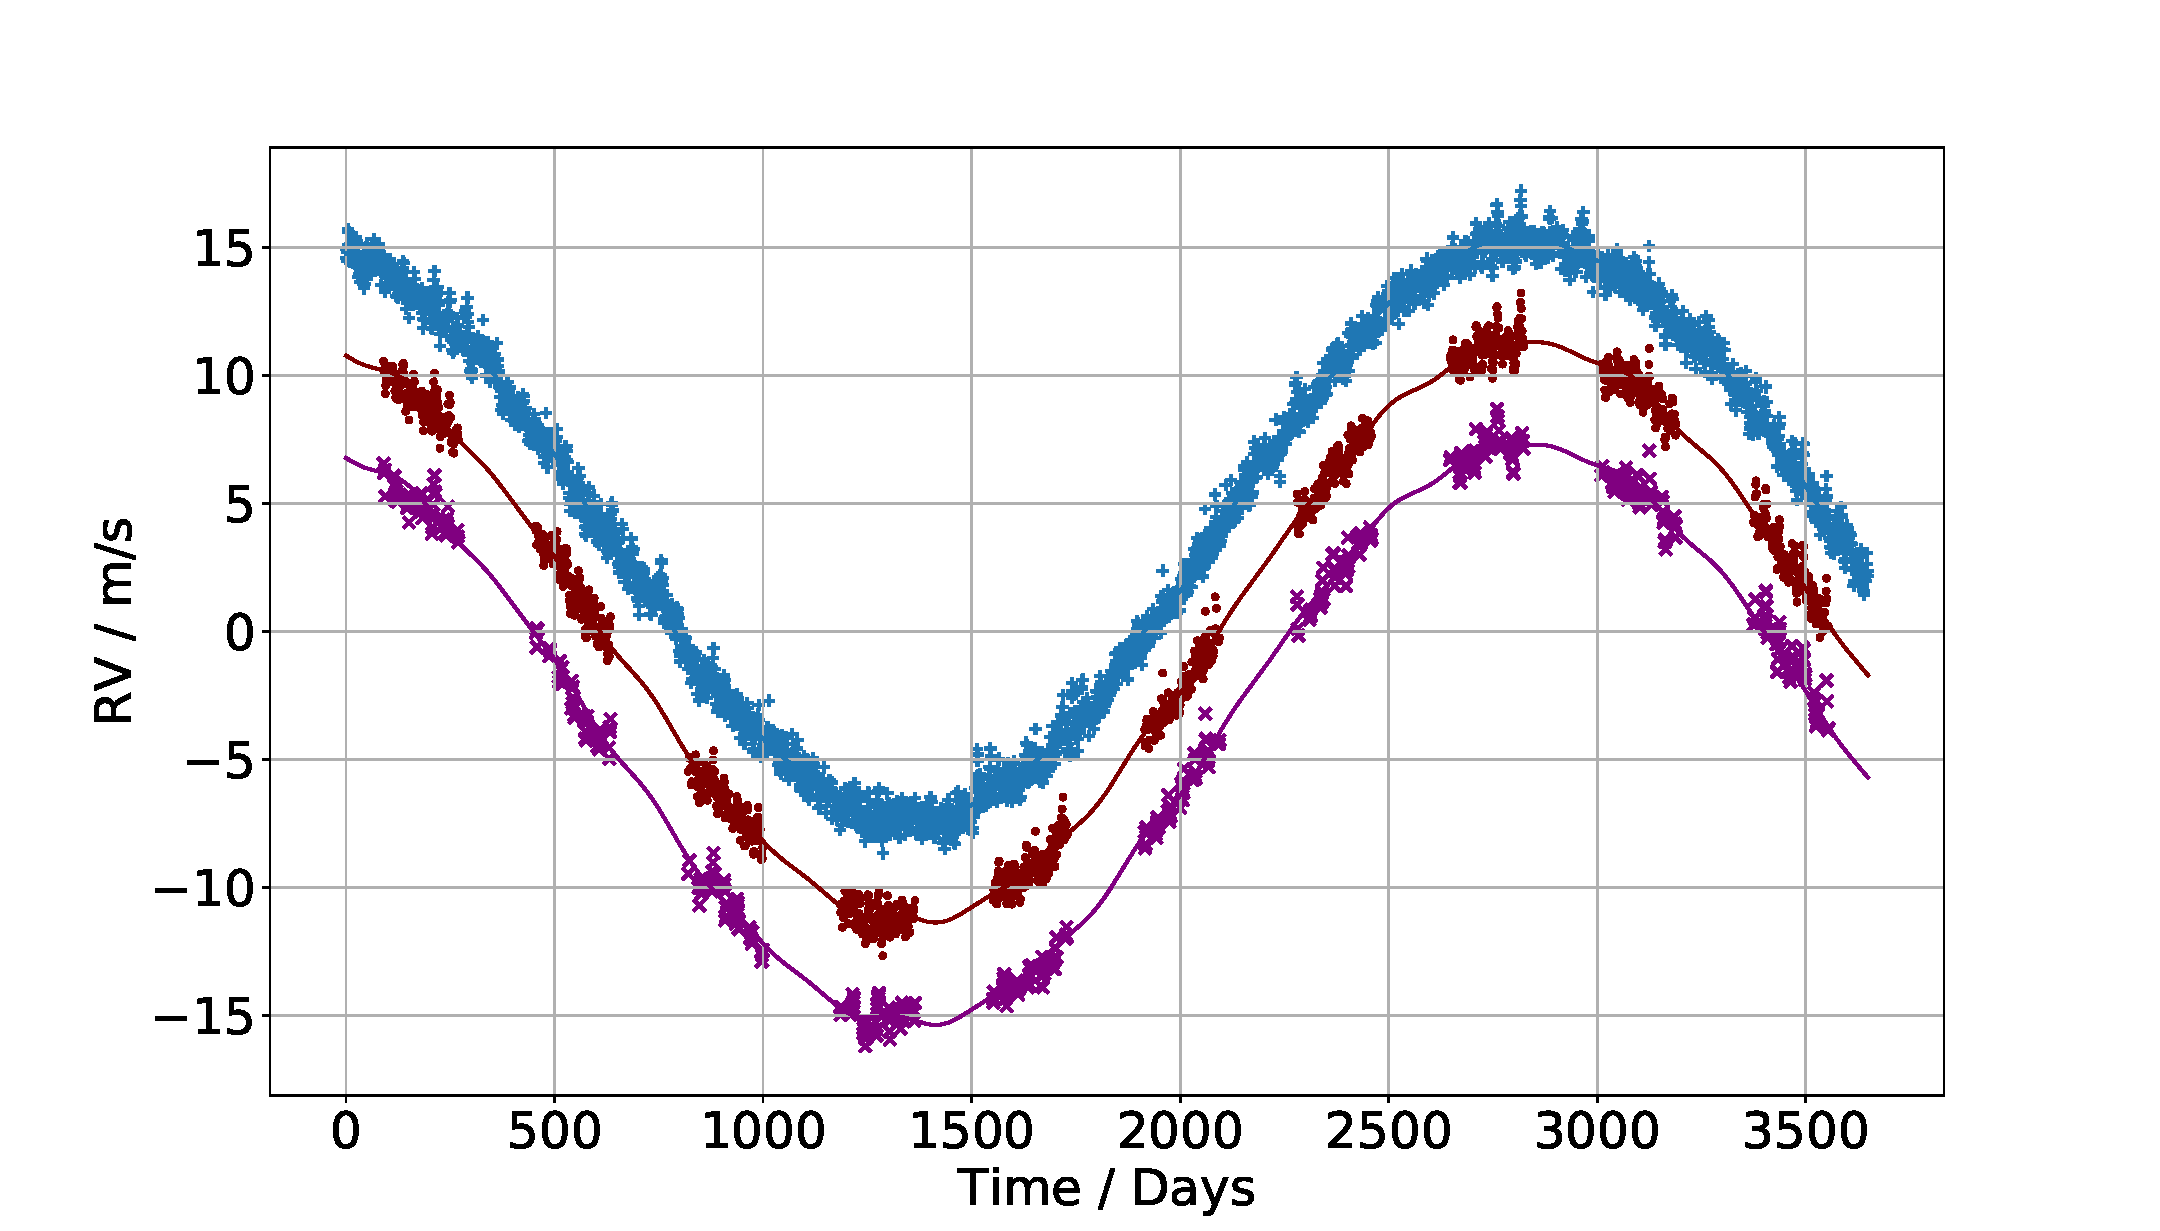
\includegraphics[width=\textwidth]{figures/rv_full.pdf}
\end{frame}

\begin{frame}
  \frametitle{Exoplanets}
  \framesubtitle{Nested sampling in action}
  \begin{itemize}
      \item Simple radial velocity model
          \begin{equation}
              \nu(t;\theta) = \sum_{p=1}^N K_p \sin(\omega_p t + \phi_p)\nonumber
          \end{equation}
      \item Fit each model to data.
      \item Posteriors on model parameters $[(K_p,\omega_p,\phi_p),p=1\cdots N]$ quantify knowledge of system characteristics.
      \item Evidences of models determine relative likelihood of number of planets in system
  \end{itemize}
\end{frame}


\begin{frame}
    \frametitle{Cosmology}
    \framesubtitle{Another example.}

    \[\lik(\Theta) = P(D|\Theta,M)\]
    \begin{align}
        \onslide<2->{D =& \{C_\ell\only<6->{^\text{(Planck)}}\}} 
        \onslide<15->{+\{\text{LSS}\}} 
        \onslide<16->{+\{\text{``Big Data''}\}}
        \nonumber\\
        \onslide<3->{M =& \Lambda\text{CDM}} 
        \onslide<9->{+ \text{extensions} }
        \nonumber\\
        \onslide<4->{\Theta =& \Theta_{\Lambda \text{CDM}}} \onslide<7->{+ \Theta_\text{Planck}} \onslide<10->{+ \Theta_\text{extensions}}\nonumber\\
        \onslide<5->{\Theta_{\Lambda \text{CDM}} =& ( \Omega_b h^2, \Omega_c h^2, 100\theta_{MC}, \tau, {\rm{ln}}(10^{10} A_s), n_s) \nonumber\\}
        \onslide<8->{\Theta_\text{Planck} =& (y_{\rm cal}, A^{CIB}_{217}, \xi^{tSZ-CIB}, A^{tSZ}_{143}, A^{PS}_{100}, A^{PS}_{143}, A^{PS}_{143\times 217}, A^{PS}_{217},\nonumber\\
        &A^{kSZ}, A^{{\rm dust}TT}_{100}, A^{{\rm dust}TT}_{143}, A^{{\rm dust}TT}_{143\times 217}, A^{{\rm dust}TT}_{217}, c_{100}, c_{217}) \nonumber\\}
        \onslide<11->{\Theta_\text{extensions} =& (
                n_{\rm run}
                \only<12->{,n_{\rm run,run}}
                \only<13->{,w}
                \only<14->{,\Sigma m_\nu, m_{\nu,{\rm{sterile}}}^{\rm{eff}}}
        ) \nonumber}
    \end{align}

    \begin{itemize}
        \item<17->{Parameter estimation: $L, \pi \to \mathcal{P}$: model parameters}
        \item<17->{Model comparison: $L, \pi \to Z$: how good model is}
    \end{itemize}

\end{frame}


\begin{frame}
  \frametitle{Nested Sampling in action}
  \framesubtitle{Primordial power spectrum $\PR(k)$ reconstruction}


  \resizebox{\textwidth} {!} {%
    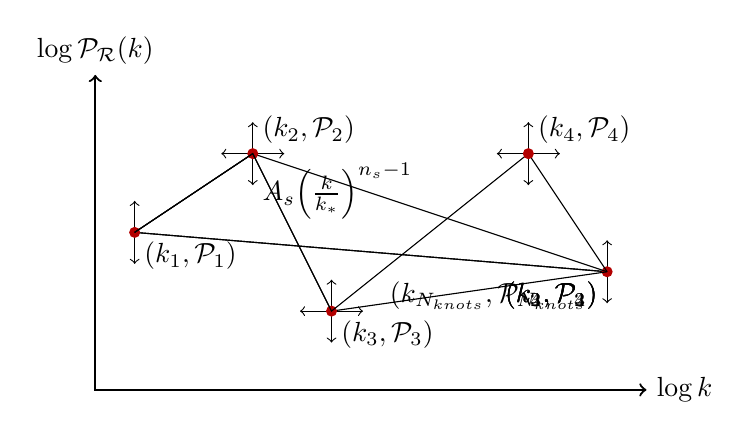
\begin{tikzpicture}
    % width of axes
      \def\xwidth{7}
      \def\ywidth{4}
    % min coordinate
      \def\xmn{0.5}
      \def\ymn{2}
    % start coordinate
      \def\xstart{2}
      \def\ystart{3}
    % middle coordinate
      \def\xmid{3}
      \def\ymid{1}
    % end coordinate
      \def\xend{5.5}
      \def\yend{3}
    % max coordinate
      \def\xmx{6.5}
      \def\ymx{1.5}

    % length of crosses
      \def\croslen{0.4}


    % Draw axes
      \draw [<->,thick] (0,\ywidth) node (yaxis) [above] {$\log\PR(k)$}
      |- (\xwidth,0) node (xaxis) [right] {$\log k$};
    % Draw limits
      %\draw [-,dashed] (\xmn,0) node[below] {$\log_{10}k_1$} -- (\xmn,\ywidth) ;
      %\draw [-,dashed] (\xmx,0) node[below] {$\log_{10}k_N$} -- (\xmx,\ywidth) ;

      \draw<1> (\xmn,\ymn) -- (\xmx,\ymx);
      \draw<1> (\xstart,\ystart) node[below right] {$A_s {\left(\frac{k}{k_*}\right)}^{n_s-1}$};

    % Draw the line joining start and end

      \coordinate (mn) at (\xmn,\ymn);
      \coordinate (start) at (\xstart,\ystart);
      \coordinate (mid) at (\xmid,\ymid);
      \coordinate (end) at (\xend,\yend);
      \coordinate (mx) at (\xmx,\ymx);
      \draw<2> (mn) -- (mx);
      \draw<2-> (mn) node[below right]    {$(k_1,\Pknotj{1})$};
      \draw<2> (mx) node[below left]     {$(k_{2},\Pknotj{{2}})$};
      \onslide<2->{\movablevert{mn}};
      \onslide<2->{\movablevert{mx}};

      \draw<3> (mn) -- (start) -- (mx);
      \onslide<3->{\movablecross{start}};
      \draw<3-> (start) node[above right] {$(k_2,\Pknotj{2})$};
      \draw<3> (mx) node[below left]     {$(k_{3},\Pknotj{{3}})$};
 
      \draw<4> (mn) -- (start) -- (mid) -- (mx);
      \onslide<4->{\movablecross{mid}};
      \draw<4-> (mid) node[below right] {$(k_3,\Pknotj{3})$};
      \draw<4> (mx) node[below left]     {$(k_{4},\Pknotj{{4}})$};

      \draw<5-> (mn) -- (start) -- (mid) -- (end) -- (mx);
      \onslide<5->{\movablecross{end}};
      \draw<5-> (end) node[above right] {$(k_4,\Pknotj{4})$};
      \draw<5-> (mx) node[below left]     {$(k_{\Nknots},\Pknotj{{\Nknots}})$};


      %\draw<2-> (\xmn,\ymn) coordinate (mn) -- (\xstart,\ystart) coordinate (start) -- (\xmid,\ymid) coordinate (mid) --  (\xend,\yend) coordinate(end) -- (\xmx,\ymx) coordinate(mx);

    % Draw the point labels
      %\draw<2-> (mn) node[below right]    {$(k_1,\Pknotj{1})$};
      %\draw<2-> (start) node[above right] {$(k_2,\Pknotj{2})$};
      %\draw<2-> (mid) node[below right]   {$(k_3,\Pknotj{3})$};
      %\draw<2-> (end) node[above right]   {$(k_4,\Pknotj{4})$};
      %\draw<2-> (mx) node[below left]     {$(k_{\Nknots},\Pknotj{{\Nknots}})$};

    % Draw a dashed line indicating the coordinate names
      %\draw[dashed] (yaxis |- start) node[left] {$y_{1}$}
      %-| (xaxis -| start) node[below] {$x_1$};
      %\draw[dashed] (yaxis |- mid) node[left] {$y_{2}$}
      %-| (xaxis -| mid) node[below] {$x_2$};
      %\draw[dashed] (yaxis |- end) node[left] {$y_{N}$}
      %-| (xaxis -| end) node[below] {$x_N$};
      %\draw  (xaxis -| start) node[below] {$\log_{10}k_2$};
      %\draw  (xaxis -| mid) node[below] {$\log_{10}k_3$};
      %\draw  (xaxis -| end) node[below] {$\log_{10}k_4$};

      % Draw the crosses
      %\onslide<2->{\movablevert{mn}
      %\movablecross{start}
      %\movablecross{mid}
      %\movablecross{end}
      %\movablevert{mx}
    %};

    % put some ellipses in between the start and end point

    \end{tikzpicture}

  }

\end{frame}
%
%
%%\begin{frame}
%%  \frametitle{Planck data}
%%  \framesubtitle{Primordial power spectrum $\PR(k)$ reconstruction}
%%  \begin{itemize}
%%    \item<2-> Temperature data TT+lowP
%%    \item<3-> Foreground $(14)$ \& cosmological $(4 +2*\Nknots-2)$  parameters
%%    \item<4-> Marginalised plots of $\PR(k)$
%%    \item<5->
%%      \[ \prob(\PR|k,\Nknots) = \int \delta(\PR-f(k;\theta))\posterior(\theta)d\theta \]
%%  \end{itemize}
%%\end{frame}
%
%
%
\begin{frame}
  \frametitle<1>{0 internal knots}
  \frametitle<2>{1 internal knots}
  \frametitle<3>{2 internal knots}
  \frametitle<4>{3 internal knots}
  \frametitle<5>{4 internal knots}
  \frametitle<6>{5 internal knots}
  \frametitle<7>{6 internal knots}
  \frametitle<8>{7 internal knots}
  \frametitle<9>{8 internal knots}
  \frametitle<10>{Bayes Factors}
  \frametitle<11>{Marginalised plot}
  \framesubtitle{Primordial power spectrum $\PR(k)$ reconstruction}


  \begin{center}
    \includegraphics<1>[width=0.8\textwidth]{figures/0TT_fgivenx}
    \includegraphics<2>[width=0.8\textwidth]{figures/1TT_fgivenx}
    \includegraphics<3>[width=0.8\textwidth]{figures/2TT_fgivenx}
    \includegraphics<4>[width=0.8\textwidth]{figures/3TT_fgivenx}
    \includegraphics<5>[width=0.8\textwidth]{figures/4TT_fgivenx}
    \includegraphics<6>[width=0.8\textwidth]{figures/5TT_fgivenx}
    \includegraphics<7>[width=0.8\textwidth]{figures/6TT_fgivenx}
    \includegraphics<8>[width=0.8\textwidth]{figures/7TT_fgivenx}
    \includegraphics<9>[width=0.8\textwidth]{figures/8TT_fgivenx}
    \includegraphics<10>[width=0.8\textwidth]{figures/Bayes_TT.pdf}
    \includegraphics<11>[width=0.8\textwidth]{figures/combined_fgivenx.pdf}

  \end{center}
\end{frame}
\begin{frame}
  \frametitle<1>{COBE (pre-2002)}
  \frametitle<2>{COBE et al (2002)}
  \frametitle<3>{WMAP (2012)}
  \frametitle<4>{Planck (2013)}
  \frametitle<5>{Planck (2015)}
  \framesubtitle{Primordial power spectrum $\PR(k)$ reconstruction}


  \begin{center}
    \includegraphics<1>[width=0.6\textwidth]{figures/cobe}
    \includegraphics<2>[width=0.6\textwidth]{figures/pre_WMAP}
    \includegraphics<3>[width=0.6\textwidth]{figures/WMAP}
    \includegraphics<4>[width=0.6\textwidth]{figures/planck_2013}
    \includegraphics<5>[width=0.6\textwidth]{figures/planck_2015}

  \end{center}
\end{frame}

\begin{frame}
    \frametitle{Unweaving runs}
    \framesubtitle{Advances in nested sampling}
    \begin{itemize}
        \item John Skilling noted that two nested sampling runs can be combined in likelihood order to produce a valid run with a larger number of live points.
        \item The reverse is also true (Higson 1704.03459).
        \item In general, a run with $n$ live points can be ``unweaved'' into $n$ runs with a single live point.
        \item Useful for providing convergence diagnostics and better parameter estimation.
    \end{itemize}
\end{frame}


\begin{frame}
  \frametitle{Dynesty}
  \framesubtitle{Advances in nested sampling (arXiv:1704.03459)}
  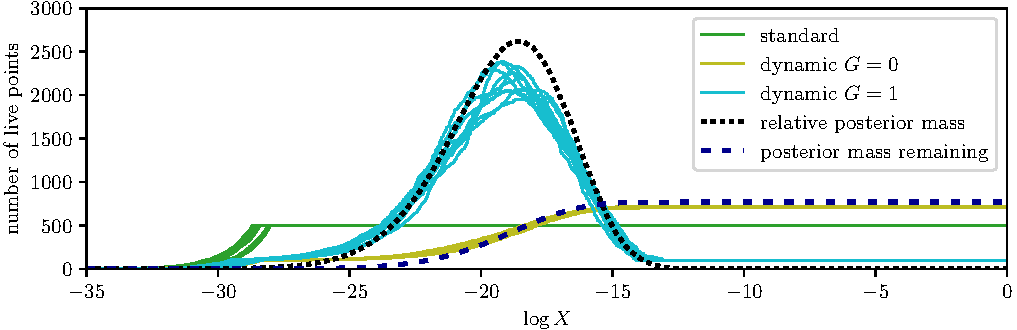
\includegraphics[width=\textwidth]{figures/dynesty.pdf}
  The number of live points can be varied dynamically in order to oversample regions of interest
\end{frame}

\begin{frame}
    \frametitle{Multi-temperature sampling}
    \framesubtitle{Advances in nested sampling}
    \begin{itemize}
        \item By compressing from prior to posterior, Nested Sampling's weighted samples are fundamentally different from traditional MCMC.
        \item Nested sampling tails and peaks equally.
        \item We can define the ``temperature'' of a distribution in analogy with thermodnyamics:
            \begin{equation}
                \log L \sim E \Rightarrow P \propto e^{-\beta E} = e^{-E/kT},\quad \beta = 1\nonumber
            \end{equation}
        \item Sampling at different temperatures can be useful for exploring tails.
        \item Nested sampling runs give you the full partition function $\log Z(\beta)$.
    \end{itemize}
\end{frame}

\begin{frame}
    \frametitle{Nested importance sampling}
    \framesubtitle{Future research}
    \begin{itemize}
        \item Much of the time spent in a nested sampling run is spent ``compressing the tails''.
        \item Sometimes we have a-priori good knowledge of the posterior bulk (analagous to an MCMC proposal distribution).
        \begin{align}
            Z_0 &= \int L(\theta) \pi_0(\theta) d\theta, \qquad
            Z_1 = \int L(\theta) \pi_1(\theta) d\theta \nonumber\\
            &= \int L(\theta)\pi_1(\theta) \frac{\pi_0(\theta)}{\pi_1(\theta)} d\theta
            = \left\langle \frac{\pi_0(\theta)}{\pi_1(\theta)} \right\rangle_{P_1}  \nonumber
        \end{align}
        \item This importance weighting only works if you have a lot of tail samples.
    \end{itemize}
\end{frame}

\begin{frame}
    \frametitle{$N$-$\sigma$ contours}
    \framesubtitle{Future research}
    \begin{itemize}
        \item Traditional posterior samples only allow you to plot contours out to 2-3$\sigma$.
        \item Nested sampling fully samples the tails, so in theory one could do $20\sigma$ contours.
        \item Requires further thought in alternatives to kernel density estimation.
    \end{itemize}
\end{frame}

%\begin{frame}
%    \frametitle{PolyChord 2.0}
%    \framesubtitle{Advances in nested sampling}
%\end{frame}

\begin{frame}[label=further_reading]
    \frametitle{Further reading}
    \centerline{%
        \hfill{}
        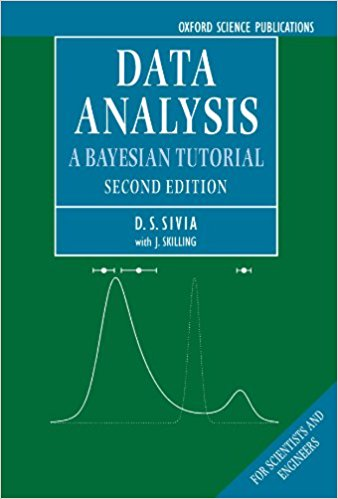
\includegraphics[height=0.7\textheight]{./figures/sivia_skilling.jpg}
        \hfill{}
        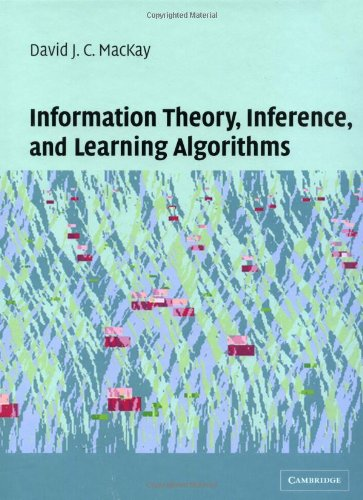
\includegraphics[height=0.7\textheight]{./figures/mackay.jpg}
        \hfill{}
    }
    \begin{itemize}
        \item Data analysis: A Bayesian Tutorial (Sivia \& Skilling)
        \item Information Theory, Inference and Learning Algorithms (Mackay)
    \end{itemize}
\end{frame}



\end{document}
